%
% gps.tex
%
% (c) Tabea Méndez und Christian Schmid, HSR
%

\chapter{Global Positioning System (GPS) als Optimierungsproblem}
\rhead{GPS als Optimierungsproblem}

\chapterauthor{Tabea M\'endez und Christian Schmid}

\begin{refsection}

Das Global Positioning System ist heute weit herum bekannt. Es
erm"oglicht die satellitengest"utzte Positionsbestimmung und erreicht
aktuell eine garantierte Genauigkeit von 7.8 Metern in 95\% der Messungen
\cite{gps:wiki}. Dies erlaubt unglaublich vielf"altige
Anwendungen, angefangen bei der Navigation, "uber Landesvermessung bis
hin zur Analysierung des Zugverhaltens von V"ogeln, welche mit einem
kleinen Sender ausger"ustet wurden.

Diese Arbeit befasst sich mit der Optimierung der Positionsberechnung
anhand der GPS-Daten welche von den Satelliten empfangen werden. Dazu
wird zuerst die grundlegende Funktionsweise sowie die technischen und
mathematischen Herausforderungen des Systems beschrieben.
	
\subsection{Funktionsweise des GPS-Systems}
Das GPS-System basiert auf mehreren Satelliten, welche die Erde auf
genau festgelegten Bahnen umkreisen. Diese Bahnen sind so angelegt, dass
zu jeder Zeit an jedem Punkt der Erde gen"ugend Satelliten f"ur eine
Positionsbestimmung empfangen werden k"onnen. Die Satelliten sind mit
(meist mehreren) genauen Atom-Uhren ausgestattet und senden ihre Position
innerhalb eines gemeinsamen Koordinatensystems sowie ihre genaue lokale
Zeit aus. Aufgrund der bekannten Position und der exakten Systemzeit zum
Sendezeitpunkt kann der Empf"anger seine Distanz zu jedem Satelliten
bestimmen. Dieser Abstand beschreibt f"ur jeden Satelliten eine Kugel
im Koordinatensystem, wobei der Sender im Kugelzentrum liegt. Sind nun
drei solche Abst"ande bzw. Kugeln bekannt, so kann sich der Empf"anger
nur an den zwei Schnittpunkten der drei Kugeln befinden. Meist kann
einer dieser Punkte vernachl"assigt werden, da er entweder unterhalb der
Erdoberfl"ache oder weit ausserhalb der Atmosph"are liegt. Die Position
des Empf"angers liesse sich also theoretisch mit den Daten von drei
Satelliten bestimmen.

F"ur die Berechnung der Signallaufzeit (und damit des Abstandes vom
Empf"anger zum Sender) muss nebst dem Sende- auch der Empfangszeitpunkt
exakt bekannt sein. Da die meisten GPS-Empf"anger jedoch nicht "uber eine
gen"ugend genaue Zeitbasis verf"ugen, muss neben den drei Raumkoordinaten
des Empfangsortes auch die genaue Zeit bestimmt werden. Um diese vier
Unbekannten zu berechnen sind also die Signale von mindestens vier
Satelliten notwendig.

Das GPS-System ist so ausgelegt, dass die Positionsbestimmung m"oglichst
zu jeder Zeit an jedem Ort m"oglich ist, auch wenn sich der Empf"anger in
einem Tal befindet und keine freie Sicht zum Horizont besteht. Deshalb
sind immer mindestens 24 Satelliten gleichzeitig aktiv, "ublicherweise
mehr. Damit lassen sich meist mehr als nur vier Satelliten f"ur die
Positionsbestimmung nutzen. Da aber nur vier Unbekannte zu bestimmen
sind wird das Gleichungssystem "uberbestimmt. Mit diesem Überfluss an
Informationen l"asst sich die Positionsbestimmung aber markant verbessern,
indem m"ogliche Fehler in den einzelnen empfangenen Signalen weniger
ins Gewicht fallen.

\subsection{Fehlereinfl"usse auf die Positionsberechnung}
Die Technik des GPS-Systems bietet mehrere Fehlerquellen, welche die
exakte Positionsbestimmung behindern k"onnen. Gegenstand dieser Arbeit
soll nicht die Verhinderung oder Kompensation dieser Fehler sein, sondern
die Optimierung der Berechnung der Position. Dabei ist es unerheblich,
woher die Fehlereinfl"usse stammen, sie sollen das Endresultat nur
m"oglichst wenig beeinflussen. Sofern die Qualit"at jedes empfangenen
Datenpakets bekannt ist kann es bei einem "uberbestimmten System
entsprechend mehr oder weniger stark gewichtet werden. Die GPS-Daten
welche die Satelliten aussenden enthalten eine solche Qualit"atsangabe,
da die Satelliten selbst in der Lage sind, zu erkennen, wie viel sie
beispielsweise von ihrer Soll-Position abweichen oder ob ihre Zeitbasis
noch korrekt ist. Weiter kann auch der Empf"anger eine Qualit"atsanalyse
vornehmen. So l"asst die Signalst"arke eines Signals beispielsweise
R"uckschl"usse darauf zu, ob das Signal direkt empfangen oder von einer
Oberfl"ache reflektiert wurde. Wird die Empfangsst"arke eines Signals
"uber eine Zeit lang beobachtet, so erlaubt auch dies eine Beurteilung
des Signalwegs. Da die Position des Senders im Signal mitgeteilt wird
k"onnen auch Satelliten, welche tief "uber dem Horizont liegen weniger
stark gewichtet werden, da ihr Signal einen weiteren Weg durch die
Atmosph"are zur"uckgelegt hat und deshalb die Signallaufzeit weniger genau
stimmen d"urfte, als wenn das Signal senkrecht oberhalb des Empf"angers
ausgesendet wurde.

\section{Grundlegende Positionsberechnung}
F"ur jeden empfangenen Satelliten kann eine Gleichung aufgestellt
werden, in welcher seine Position in Relation zum Abstand zum Empf"anger
gestellt wird.
\[
(x_i - x)^2 + (y_i - y)^2 + (z_i - z)^2 - (t - t_i)^2\cdot c^2 = 0
\]
$x_i, y_i, z_i$ stehen dabei f"ur die Raumkoordinaten des Senders,
$x, y, z$ f"ur diejenigen des Empf"angers. Die ersten drei Quadrate
ergeben aufsummiert den Abstand zwischen Sender und Empf"anger. Das
vierte Quadrat wiederum errechnet den Abstand aus der Zeitdifferenz,
multipliziert mit der Geschwindigkeit mit welcher sich die Signale
ausbreiten. Da diese beiden Distanzen gleich gross sein m"ussen werden
sie voneinander subtrahiert und sollen 0 ergeben.

Sind nun die Daten von nur vier Satelliten bekannt, so kann ein
Gleichungssystem mit 4 Gleichungen und 4 Unbekannten aufgestellt und
eindeutig gel"ost werden.
\begin{align*}
	(x_1 - x)^2 + (y_1 - y)^2 + (z_1 - z)^2 - c^2\cdot(t - t_1)^2 &= 0\\
	(x_2 - x)^2 + (y_2 - y)^2 + (z_2 - z)^2 - c^2\cdot(t - t_2)^2 &= 0\\
	(x_3 - x)^2 + (y_3 - y)^2 + (z_3 - z)^2 - c^2\cdot(t - t_3)^2 &= 0\\
	(x_4 - x)^2 + (y_4 - y)^2 + (z_4 - z)^2 - c^2\cdot(t - t_4)^2 &= 0\\
\end{align*}
Werden nun mehr als vier Satelliten empfangen, so ist das
Gleichungssystem "uberbestimmt. Damit l"auft die Positionsbestimmung
auf ein Optimierungsproblem heraus.

\begin{figure}[ht!]\centering
	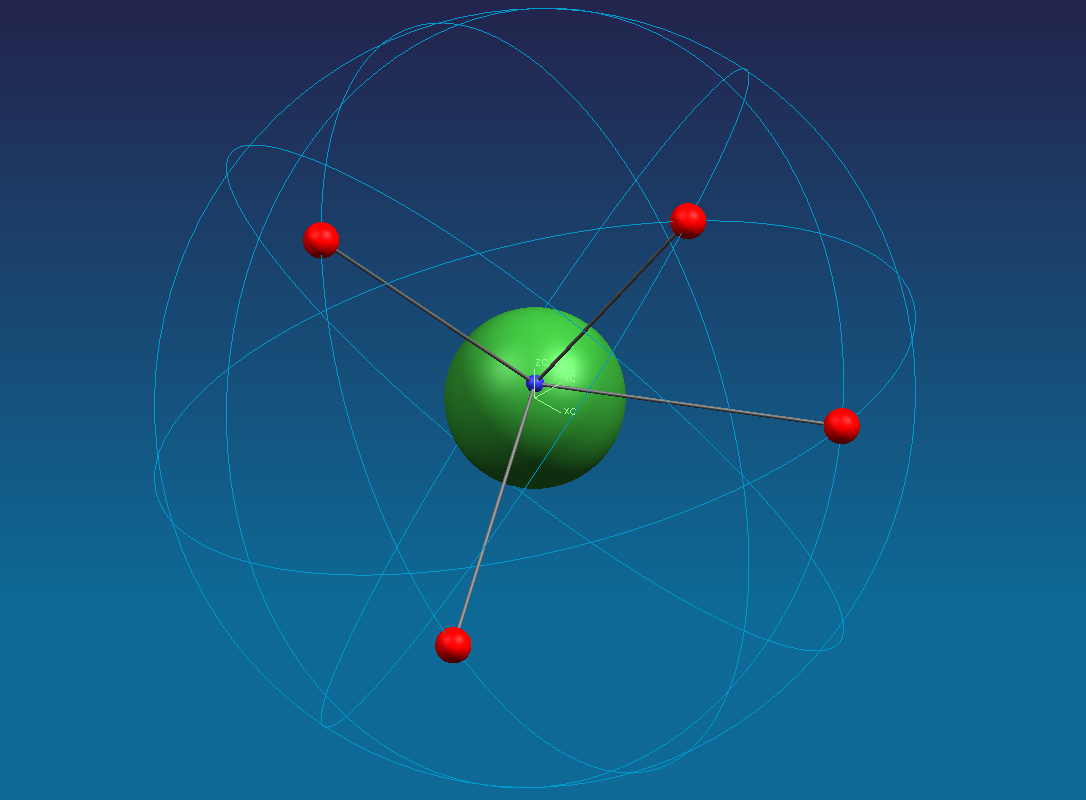
\includegraphics[scale = 0.3]{gps/gps.png}
	\caption{Satellitenkonstellation}
	\label{fig. satellitenkonstellation}
\end{figure}

\section{Optimierungsproblem}
Wenn die eigene Position mit Hilfe von GPS-Satelliten bestimmt werden
soll, k"onnen in den meisten F"allen von mehr als vier Satelliten Daten
empfangen werden. Dadurch entsteht ein "uberbestimmtes Gleichungssystem
mit $4$ unbekannten Variablen $(x_0,y_0,z_0,t_0)$ und $n$ Gleichungen
($n = $ Anzahl empfangene Satellitendaten). Das Optimierungsproblem liegt
dann darin, aus den empfangen Satellitendaten die Position zu finden,
die am besten stimmt, bzw. den Ort an dem der quadratische Fehler am
kleinsten ist (``method of least squares'').

\subsection{Zielfunktion}
Die Zielfunktion, die es dabei zu minimieren gilt, lautet folgendermassen:
\[
f(x,y,z,t)
=
\sum_{i=1}^{n}\left[
\underbrace{(x_i-x)^2 + (y_i-y)^2 + (z_i-z)^2}_{\text{Distanz aus Raumkoordinaten}}
-
\underbrace{c^2 (t-t_i)^2}_{\text{Distanz aus Zeit}}\right]^2
\]
Die Bedeutung der Variablen in der Summe ist wie folgt:
\begin{center}
\begin{tabular}{ll}
Anzahl Satelliten: $\quad$& $n$\\
Satellitendaten: $\quad$& $x_i$, $y_i$, $z_i$ und $t_i$\\
Lichtgeschwindigkeit: $\quad$& $c$\\
\end{tabular}
\end{center}
Bei dieser Zielfunktion werden die Fehler der einzelnen Satelliten
quadriert und anschliessend aufsummiert. Durch das Quadrieren wird
verhindert, dass sich die Fehler der Satelliten gegenseitig kompensieren
k"onnen. Wird nun ein Punkt gefunden an dem die Zielfunktion und damit
der quadrierte und aufsummierte Fehler der Satelliten minimal wird,
so wird in diesem Punkt auch der Positionsfehler minimal. Diesen Punkt
gilt es also zu finden.

\subsection{Minimum der Zielfunktion finden}\label{Minimum der ZF}
Um die Extremalstellen (Maxima oder Minima) der Zielfunktion $f$
zu finden, muss der Gradient von $f$ gleich Null gesetzt werden. Der
Gradient ist ein Vektor, welcher die ersten partiellen Ableitungen
der Zielfunktion beinhaltet und immer in die Richtung des steilsten
Anstiegs zeigt. Ist nun der Gradient, und damit der steilste Anstieg in
einem Punkt Null, so handelt es sich bei diesem Punkt um ein Maximum,
ein Minimum oder einen Sattelpunkt.

\[
\nabla f
=
\begin{bmatrix}
\frac{\partial f}{\partial x}\\
\frac{\partial f}{\partial y}\\
\frac{\partial f}{\partial z}\\
\frac{\partial f}{\partial t}
\end{bmatrix}
=
\begin{bmatrix}
\sum\limits_{i=1}^{n}-4\,(x_i-x)\bigl((x_i - x)^2 + (y_i - y)^2 + (z_i - z)^2 - c^2(t - t_i)^2 \bigr)\\
\sum\limits_{i=1}^{n}-4\,(y_i-y)\bigl((x_i - x)^2 + (y_i - y)^2 + (z_i - z)^2 - c^2(t - t_i)^2 \bigr)\\
\sum\limits_{i=1}^{n}-4\,(z_i-z)\bigl((x_i - x)^2 + (y_i - y)^2 + (z_i - z)^2 - c^2(t - t_i)^2 \bigr)\\
\sum\limits_{i=1}^{n}-4 c^2(t-t_i)\bigl((x_i - x)^2 + (y_i - y)^2 + (z_i - z)^2 - c^2(t - t_i)^2\bigr)
\end{bmatrix}
=
\begin{bmatrix} 0 \\ 0 \\ 0 \\ 0 \end{bmatrix}
\]
		Zum l"osen dieses nicht linearen Gleichungssystems ist das Newton-Verfahren geeignet.

\subsection{Newton-Verfahren}
Die Idee des Newton-Verfahrens ist, die Funktion fortlaufend durch
ihre Linearisierung zu approximieren und dann das vereinfachte lineare
Gleichungssystem zu l"osen.

Zur Illustration wird das Newton-Verfahren vorerst
an einem 1-dimensionalen Beispiel gezeigt (Abbildung
\ref{fig. 1dim-Bsp-Newton}).

Als erstes muss ein Startpunkt gew"ahlt werden, in welchem die
Funktion $f(x)$ linearisiert wird. Im gezeigten Beispiel ist dies
der Punkt $P_0$. Danach wird das linearisierte Gleichungssystem
$|g_0(x)=0|$ gel"ost. Dies liefert einen neuen Punkt $P_1$, mit
dem das Ganze wiederholt wird. Wiederum die Funktion $f(x)$ im
Punkt $P_1$ linearisieren, dann das linearisierte Gleichungssystem
$|g_1(x)=0|$ l"osen und wiederum im berechneten neuen Punkt $P_2$
linearisieren. Mit jedem Iterationsschritt wird die L"osung verbessert,
wobei der Verbesserungsschritt dabei immer kleiner wird. Die Iteration
kann abgebrochen werden, sobald der Verbesserungsschritt gen"ugend klein
und damit die L"osung gen"ugend genau ist.

		\begin{figure}[ht!]\centering
 			\begin{tikzpicture}[>=latex',scale=1.4]
				\draw[->] (0.3,0) -- (4.9,0)node[right] {$x$};
				\draw[->] (0.5,-0.2) -- (0.5,3) node[above] {$y$};
				\draw[smooth,samples=100,domain=0.3:4.8, black, line width=0.75 ] plot (\x,{(0.4*\x-0.1)*(0.4*\x-0.1)-0.3})node[above]{\footnotesize $f(x)$}; 
				\draw[smooth,samples=100,domain=2:4.8, gray, line width=0.5 ] plot (\x,{1.36*(\x-4.5)+2.59})node at(3.35,0.5){\footnotesize $g_0(x)$};
				\filldraw[red!70!black] (4.5,0)circle(1.5pt)nodeat(4.5,-0.3){\footnotesize $P_0$};
				\draw[->, line width=0.5, red!70!black, dashed] (4.5,0)--(4.5,2.59);
				\filldraw[red!70!black] (4.5,2.59)circle(1.5pt);
				\draw[smooth,samples=100,domain=1:4, gray, line width=0.5 ] plot (\x,{0.750588*(\x-2.59559)+0.580285})node at(1,-0.8){\footnotesize $g_1(x)$};
				\filldraw[red!70!black] (2.59559,0)circle(1.5pt)nodeat(2.7,-0.3){\footnotesize $P_1$};
				\draw[->, line width=0.5, red!70!black, dashed] (2.59559,0)--(2.59559,0.580285);
				\filldraw[red!70!black] (2.59559,0.580285)circle(1.5pt);
				\draw[smooth,samples=100,domain=0.6:2.5, gray, line width=0.5 ] plot (\x,{0.503194*(\x-1.82248)+0.095631})node at(0.3,-0.6){\footnotesize $g_2(x)$};
				\filldraw[red!70!black] (1.82248,0)circle(1.5pt)node at(1.9,-0.3){\footnotesize $P_2$};
				\filldraw[red!70!black] (1.82248,0.095631)circle(1.5pt);
				\filldraw[green!70!black!] (1.63243,0)circle(1.5pt) node at(1.1,0.3) {\footnotesize L"osung};
 			\end{tikzpicture}
 			\caption{Newton-Verfahren}
			\label{fig. 1dim-Bsp-Newton}
 		\end{figure}
 
\subsubsection{Schleifen beim Newton-Verfahren}
Das Newton-Verfahren f"uhrt leider nicht in jedem Fall zu einer
L"osung. Je nach dem wie die Funktion aussieht, ist es beispielsweise
m"oglich, dass der Newton-Algorithmus in einer Schliefe h"angen
bleibt, wie das in der Grafik gezeigt ist. Dieses Problem ist bei der
L"osungsfindung zu ber"ucksichtigen.
\begin{figure}[ht!]\centering
	\begin{tikzpicture}[>=latex', scale=0.8]
		\draw[->] (-2.3,0) -- (2.5,0)node[right] {$x$};
		\draw[->] (0,-1.5) -- (0,1.5) node[above] {$y$};
		\draw[smooth,samples=100,domain=-2.3:2.3, gray, line width=0.75 ] plot (\x,{0.5*\x+1});			
		\draw[smooth,samples=100,domain=-2.3:2.4, gray, line width=0.75 ] plot (\x,{0.5*\x-1});			
		\draw[smooth,samples=100,domain=-2.5:2.5, black, line width=1 ] plot (\x,{2.15*sin((\x)*105/pi)});
		\draw[->,red!70!black, line width=0.75,dashed] (2,0) -- (2,2);
		\draw[->,red!70!black, line width=0.75,dashed] (-2,0) -- (-2,-2);
		\filldraw[red!70!black] (-2,0)circle(2pt);
		\filldraw[red!70!black] (2,0)circle(2pt);
		\filldraw[red!70!black] (-2,-2)circle(2pt);
		\filldraw[red!70!black] (2,2)circle(2pt);
% 					\draw[white](-1,-4)--(1,-4);
	\end{tikzpicture}
	\caption{Schleifen beim Newton-Verfahren}
	\label{fig. Schleife}
\end{figure}

\subsubsection{Anwendung des Newton-Verfahren auf das GPS-Optimierungsproblem}
Wird nun das Newton-Verfahren auf das GPS-Optimierungsproblem angewendet,
funktioniert das folgendermassen:
\begin{enumerate}
\item Geeigneten Startpunkt $p_0 = (x_0,\,y_0,\,z_0,\,t_0)$ w"ahlen.
\item Gleichungssystem in diesem Punkt linearisieren.\\[0.2cm]
\begin{align*}
&\nabla f (x_j,y_j,z_j,t_j) = \nabla f (p_j) =  
\begin{bmatrix}
f_x(p_j) \\
f_y(p_j) \\
f_z(p_j) \\
f_t(p_j)
\end{bmatrix} \approx
\begin{bmatrix} g_x(p_j) \\
g_y(p_j) \\
g_z(p_j) \\
g_t(p_j)
\end{bmatrix}\\
&= \begin{bmatrix} f_{xx}(p_j)\, (x-x_j) + f_{xy}(p_j)\, (y-y_j) + f_{xz}(p_j)\, (z-z_j) + f_{xt}(p_j)\, (t-t_j) + f_x(p_j) \\
f_{xy}(p_j)\, (x-x_j) + f_{yy}(p_j)\, (y-y_j) + f_{yz}(p_j)\, (z-z_j) + f_{yt}(p_j)\, (t-t_j) + f_y(p_j) \\
f_{xz}(p_j)\, (x-x_j) + f_{yz}(p_j)\, (y-y_j) + f_{zz}(p_j)\, (z-z_j) + f_{zt}(p_j)\, (t-t_j) + f_z(p_j) \\
f_{xt}(p_j)\, (x-x_j) + f_{yt}(p_j)\, (y-y_j) + f_{zt}(p_j)\, (z-z_j) + f_{tt}(p_j)\, (t-t_j) + f_t(p_j) 
\end{bmatrix}\\
&= \begin{bmatrix} 
f_{xx}(p_j) &  f_{xy}(p_j) & f_{xz}(p_j) & f_{xt}(p_j)\\
f_{xy}(p_j) & f_{yy}(p_j) & f_{yz}(p_j) & f_{yt}(p_j)\\
f_{xz}(p_j) & f_{yz}(p_j) & f_{zz}(p_j) & f_{zt}(p_j)\\
f_{xt}(p_j) & f_{yt}(p_j) & f_{zt}(p_j) & f_{tt}(p_j)
\end{bmatrix} \cdot
\begin{bmatrix} 
\Delta x \\
\Delta y \\
\Delta z \\
\Delta t 
\end{bmatrix} +
\begin{bmatrix} 
f_x(p_j) \\
f_y(p_j) \\
f_z(p_j) \\
f_t(p_j) 
\end{bmatrix}
\end{align*}
\item Linearisiertes Gleichungssystem l"osen.\\[0.2cm]
\begin{align*}
\begin{bmatrix} 
f_{xx}(p_j) &  f_{xy}(p_j) & f_{xz}(p_j) & f_{xt}(p_j)\\
f_{xy}(p_j) & f_{yy}(p_j) & f_{yz}(p_j) & f_{yt}(p_j)\\
f_{xz}(p_j) & f_{yz}(p_j) & f_{zz}(p_j) & f_{zt}(p_j)\\
f_{xt}(p_j) & f_{yt}(p_j) & f_{zt}(p_j) & f_{tt}(p_j)
\end{bmatrix} \cdot
\begin{bmatrix} 
\Delta x \\
\Delta y \\
\Delta z \\
\Delta t 
\end{bmatrix} + \begin{bmatrix} 
f_x(p_j) \\
f_y(p_j) \\
f_z(p_j) \\
f_t(p_j) 
\end{bmatrix}&= \begin{bmatrix} 0 \\ 0 \\ 0 \\ 0 \end{bmatrix}
\\
\begin{bmatrix} 
f_{xx}(p_j) &  f_{xy}(p_j) & f_{xz}(p_j) & f_{xt}(p_j)\\
f_{xy}(p_j) & f_{yy}(p_j) & f_{yz}(p_j) & f_{yt}(p_j)\\
f_{xz}(p_j) & f_{yz}(p_j) & f_{zz}(p_j) & f_{zt}(p_j)\\
f_{xt}(p_j) & f_{yt}(p_j) & f_{zt}(p_j) & f_{tt}(p_j)
\end{bmatrix} \cdot \begin{bmatrix} 
\Delta x \\
\Delta y \\
\Delta z \\
\Delta t 
\end{bmatrix}&= \begin{bmatrix} 
-f_x(p_j) \\
-f_y(p_j) \\
-f_z(p_j) \\
-f_t(p_j) 
\end{bmatrix}
\end{align*}
\item Neuer Punkt berechnen.
\[
p_{j+1} = (x_j + \Delta x,\,y_j + \Delta y,\,z_j + \Delta z,\,t_j + \Delta t)
\]
\item Wieder bei Punkt 2. beginnen.
\item Solange wiederholen, bis $\Delta x$, $\Delta y$, $\Delta z$
und $\Delta t$ gen"ugend klein sind. 
\end{enumerate}

\subsection{Arten von station"aren Punkten}\label{stat_Punkte}
Wie im Abschnitt \ref{Minimum der ZF} bereits erw"ahnt, muss zum finden
der Extremalstellen der Gradient von $f$ gleich Null gesetzt werden. Dabei
k"onnen als L"osungen dieses Gleichungssystems $|\nabla f = \vec 0 |$
drei Arten von station"aren Punkten vorkommen. Zum einen Maxima oder
Minima, die f"ur Optimierungsprobleme im Allgemeinen von Bedeutung sind,
und zum anderen Sattelpunkte. Sattelpunkte sind Stellen an denen es in
gewisse Richtungen ansteigt und in andere abf"allt. Da es drei Arten von
L"osungen gibt, jedoch f"ur das GPS-Optimierungsproblem nur die Minima
von Bedeutung sind, m"ussen die anderen L"osungen ausgesondert werden. Um
bestimmen zu k"onnen, um welche L"osungsart es sich bei einem bestimmten
Punkt handelt, m"ussen die Eigenwerte $\lambda_i$ der Hesseschen Matrix
berechnet werden. Die Hessesche Matrix sieht folgendermassen aus:
\[
		H = \begin{bmatrix} 
		f_{xx}(p_L) & f_{xy}(p_L) & f_{xz}(p_L) & f_{xt}(p_L)\\
		f_{xy}(p_L) & f_{yy}(p_L) & f_{yz}(p_L) & f_{yt}(p_L)\\
		f_{xz}(p_L) & f_{yz}(p_L) & f_{zz}(p_L) & f_{zt}(p_L)\\
		f_{xt}(p_L) & f_{yt}(p_L) & f_{zt}(p_L) & f_{tt}(p_L)
		\end{bmatrix} \qquad\begin{array}{l} p_L\text{: L"osungspunkt}\end{array}
\]
Anhand der berechneten Eigenwerte kann nun die Art des station"aren
Punktes bestimmt werden.
\begin{center}
\begin{tabular}{lcllcl}
	& $\bullet$ & Minimum: & alle Eigenwerte $\lambda_i$ sind positiv: & $\Rightarrow$ & $\lambda_i > 0\quad,\forall i$\\
	& $\bullet$ & Maximum: & alle Eigenwerte $\lambda_i$ sind negativ: & $\Rightarrow$ & $\lambda_i < 0\quad,\forall i$\\
	& $\bullet$ & Sattelpunkt: & alle Eigenwerte $\lambda_i$ sind positiv oder negativ: & $\Rightarrow$ & $\lambda_i > 0 \;\lor\; \lambda_i < 0\quad,\forall i$\\
\end{tabular}
\end{center}

\subsection{Ber"ucksichtigung der Sattelpunkte beim Newton-Verfahren}
Mit dem Wissen, dass das Gleichungssystem $|\nabla f = \vec 0 |$
(Abschnitt \ref{Minimum der ZF}) als L"osungen auch Sattelpunkte liefert,
kann nun das Newton-Verfahren noch verbessert werden. Angenommen das
Newton-Verfahren liefert als L"osung kein Minimum sondern ein Sattelpunkt,
so gibt es mindestens eine Richtung, in die die Funktion abf"allt. Wird
nun der Newton-Algorithmus gezielt in diese Richtung gelenkt, so ist
es m"oglich, dass doch noch ein Minimum gefunden wird. Dabei ist die
erfolgversprechendste Richtung nat"urlich die, in die es am steilsten
abf"allt. Um diese Richtung zu finden, muss der Eigenvektor $\vec v_-$
zu einem negativen Eigenwert $\lambda_-$ gefunden werden. Der gefunde
Eigenvektor $\vec v_-$ zeigt dann in die Richtung des steilsten
Abstiegs.
\begin{align*}
H\cdot \vec v_-&= \lambda_- \cdot \vec v_-\\
\left[H-\lambda_-\cdot E\right] \cdot \vec v_-&= \vec 0
\end{align*}
Darin bedeuten:
\begin{center}
\begin{tabular}{>{$}r<{$:}l}
H&
Hessesche Matrix des Sattelpunktes (vgl. Kapitel \ref{stat_Punkte})\\
\lambda_-&
Negativer Eigenwert der Hesseschen Matrix (vgl. Kapitel \ref{stat_Punkte})\\
\vec v_-&
Eigenvektor zum Eigenwert $\lambda_-$
\end{tabular}
\end{center}
Der Eigenvektor $v_-$ zum kleinsten Eigenvektor zeigt in Richtung
des steilsten Abstiegs (Siehe Abbildung \ref{gps:Sattelpunkte}).

\begin{figure}\centering
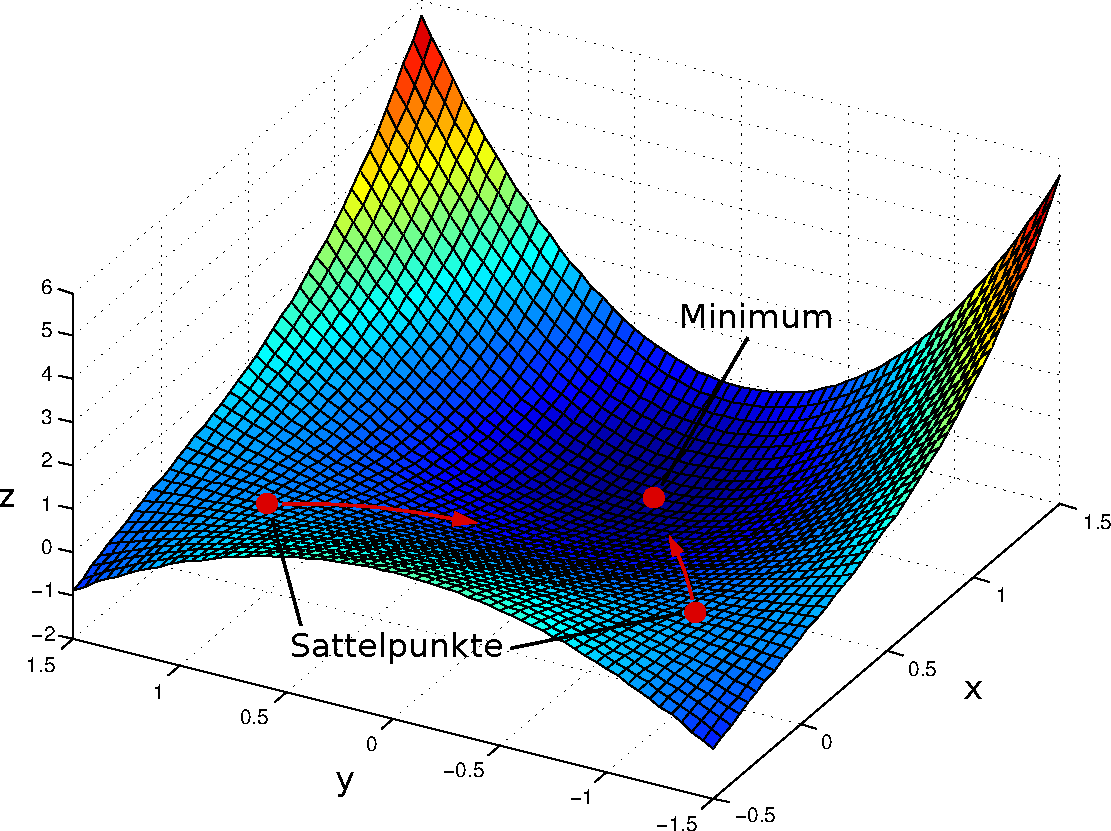
\includegraphics[scale = 0.6]{gps/sattel.pdf}
\caption{Sattelpunkte}
\label{gps:Sattelpunkte}
\end{figure}

\subsection{Gewichtung der Satelliten}
Um das Resultat der Positionsbestimmung noch zu verbessern, k"onnen die
einzelnen Satelliten, bzw. die Fehler der Satellitendaten zus"atzlich
mit einem Faktor gewichtet werden. Die Gewichtung wird zum einen aus
der Empfangsqualit"at und zum anderen aus der Genauigkeit der Daten
selber, die vom Satelliten gesendet wird, bestimmt. Die Zielfunktion
mit Gewichtungsfaktoren sieht dann wie folgt aus:
\[
f(x,y,z,t) =
\sum_{i=1}^{n}\left[\frac{1}{\sigma_i}\cdot \left((x_i-x)^2 + (y_i-y)^2 + (z_i-z)^2\;\, - c^2 (t-t_i)^2\;\right)\right]^2.
\]
Ist dabei die Standardabweichung $\sigma_i$ eines Satelliten gross, so
wird sein Gewichtungsfaktor klein und dadurch wird er bei der Berechnung
der Position weniger gewichtet.

\subsection{Zielfunktion und deren Ableitungen}
\subsubsection{Ohne Gewichtung der Satelliten}
\begin{tabular}{l}
	\textbf{Zielfunktion:}\\
	$f(x,y,z,t) = \text{\large$\sum\limits_{i=1}^{n}$}\;{\left[(x_i-x)^2 + (y_i-y)^2 + (z_i-z)^2\;\, - c^2 (t-t_i)^2\;\right]^2}$\\[0.4cm]
	\hline
	\\[-0.3cm]
	\textbf{Erste partielle Ableitungen in $x$, $y$, $z$ und $t$:}\\
	$f_x(x,y,z,t) = -4\;\text{\large$\sum\limits_{i=1}^{n}$}\;{\;(x_i-x)\left[(x_i - x)^2 + (y_i - y)^2 + (z_i - z)^2 - c^2(t - t_i)^2 \right]}$\\
	$f_y(x,y,z,t) = -4\;\text{\large$\sum\limits_{i=1}^{n}$}\;{\;(y_i-y)\left[(x_i - x)^2 + (y_i - y)^2 + (z_i - z)^2 - c^2(t - t_i)^2 \right]}$\\
	$f_z(x,y,z,t) = -4\;\text{\large$\sum\limits_{i=1}^{n}$}\;{\;(z_i-z)\left[(x_i - x)^2 + (y_i - y)^2 + (z_i - z)^2 - c^2(t - t_i)^2 \right]}$\\
	$f_t(x,y,z,t) = -4 \,c^2\;\text{\large$\sum\limits_{i=1}^{n}$}\;{\;(t-t_i)\left[(x_i - x)^2 + (y_i - y)^2 + (z_i - z)^2 - c^2(t - t_i)^2\right]}$\\[0.4cm]
	\hline
	\\[-0.3cm]
	\textbf{Zweite partielle Ableitungen in $x$, $y$, $z$ und $t$:}\\
	$f_{xx}(x,y,z,t) = 4\;\text{\large$\sum\limits_{i=1}^{n}$}\;{\;\left[3\cdot(x_i - x)^2 + (y_i - y)^2 + (z_i - z)^2 - c^2(t - t_i)^2\right]}$\\
	$f_{xy}(x,y,z,t) = 8\;\text{\large$\sum\limits_{i=1}^{n}$}\;{\;(x_i-x)(y_i-y)}$\\
	$f_{xz}(x,y,z,t) = 8\;\text{\large$\sum\limits_{i=1}^{n}$}\;{\;(x_i-x)(z_i-z)}$\\
	$f_{xt}(x,y,z,t) = 8\,c^2\;\text{\large$\sum\limits_{i=1}^{n}$}\;{\;(x_i-x)(t-t_i)}$\\[0.4cm]
%				\arrayrulecolor{gray}
	\hline
	\\[-0.3cm]
	$f_{yy}(x,y,z,t) = 4\;\text{\large$\sum\limits_{i=1}^{n}$}\;{\;\left[(x_i - x)^2 + 3\cdot(y_i - y)^2 + (z_i - z)^2 - c^2(t - t_i)^2\right]}$\\
	$f_{yz}(x,y,z,t) = 8\;\text{\large$\sum\limits_{i=1}^{n}$}\;{\;(y_i-y)(z_i-z)}$\\
	$f_{yt}(x,y,z,t) = 8\,c^2\;\text{\large$\sum\limits_{i=1}^{n}$}\;{\;(y_i-y)(t-t_i)}$\\[0.4cm]
	\hline
	\\[-0.3cm]
	$f_{zz}(x,y,z,t) = 4\;\text{\large$\sum\limits_{i=1}^{n}$}\;{\;\left[(x_i - x)^2 + (y_i - y)^2 + 3 \cdot (z_i - z)^2 - c^2(t - t_i)^2\right]}$\\
	$f_{zt}(x,y,z,t) = 8\,c^2\;\text{\large$\sum\limits_{i=1}^{n}$}\;{\;(z_i-z)(t-t_i)}$\\[0.5cm]
	\hline
	\\[-0.3cm]
	$f_{tt}(x,y,z,t) = -4\,c^2\;\text{\large$\sum\limits_{i=1}^{n}$}\;{\;\left[(x_i - x)^2 + (y_i - y)^2 + (z_i - z)^2 - 3\,c^2\cdot(t - t_i)^2\right]}$\\[0.4cm]
%				\arrayrulecolor{black}
	\hline
\end{tabular}

\subsubsection{Mit Gewichtung der Satelliten}
\begin{tabular}{l}
\textbf{Zielfunktion:}\\
$f(x,y,z,t) = \text{\large$\sum\limits_{i=1}^{n}$}\;{\left[\dfrac{1}{\sigma_i}\cdot \left((x_i-x)^2 + (y_i-y)^2 + (z_i-z)^2\;\, - c^2 (t-t_i)^2\;\right)\right]^2}$\\[0.4cm]
\hline
\\[-0.3cm]
\textbf{Erste partielle Ableitungen in $x$, $y$, $z$ und $t$:}\\[0.1cm]
$f_x(x,y,z,t) = -4\;\text{\large$\sum\limits_{i=1}^{n}$}\;{\;\dfrac{1}{{\sigma_i}^2}\,(x_i-x)\left[(x_i - x)^2 + (y_i - y)^2 + (z_i - z)^2 - c^2(t - t_i)^2 \right]}$\\[0.4cm]
$f_y(x,y,z,t) = -4\;\text{\large$\sum\limits_{i=1}^{n}$}\;{\;\dfrac{1}{{\sigma_i}^2}\,(y_i-y)\left[(x_i - x)^2 + (y_i - y)^2 + (z_i - z)^2 - c^2(t - t_i)^2 \right]}$\\[0.4cm]
$f_z(x,y,z,t) = -4\;\text{\large$\sum\limits_{i=1}^{n}$}\;{\;\dfrac{1}{{\sigma_i}^2}\,(z_i-z)\left[(x_i - x)^2 + (y_i - y)^2 + (z_i - z)^2 - c^2(t - t_i)^2 \right]}$\\[0.4cm]
$f_t(x,y,z,t) = -4 \,c^2\;\text{\large$\sum\limits_{i=1}^{n}$}\;{\;\dfrac{1}{{\sigma_i}^2}\,(t-t_i)\left[(x_i - x)^2 + (y_i - y)^2 + (z_i - z)^2 - c^2(t - t_i)^2\right]}$\\[0.4cm]
\hline
\\[-0.3cm]
\textbf{Zweite partielle Ableitungen in $x$, $y$, $z$ und $t$:}\\[0.1cm]
$f_{xx}(x,y,z,t) = 4\;\text{\large$\sum\limits_{i=1}^{n}$}\;{\;\dfrac{1}{{\sigma_i}^2}\,\left[3\cdot(x_i - x)^2 + (y_i - y)^2 + (z_i - z)^2 - c^2(t - t_i)^2\right]}$\\[0.4cm]
$f_{xy}(x,y,z,t) = 8\;\text{\large$\sum\limits_{i=1}^{n}$}\;{\;\dfrac{1}{{\sigma_i}^2}\,(x_i-x)(y_i-y)}$\\[0.4cm]
$f_{xz}(x,y,z,t) = 8\;\text{\large$\sum\limits_{i=1}^{n}$}\;{\;\dfrac{1}{{\sigma_i}^2}\,(x_i-x)(z_i-z)}$\\[0.4cm]
$f_{xt}(x,y,z,t) = 8\,c^2\;\text{\large$\sum\limits_{i=1}^{n}$}\;{\;\dfrac{1}{{\sigma_i}^2}\,(x_i-x)(t-t_i)}$\\[0.4cm]
%				\arrayrulecolor{gray}
\hline
\\[-0.3cm]
$f_{yy}(x,y,z,t) = 4\;\text{\large$\sum\limits_{i=1}^{n}$}\;{\;\dfrac{1}{{\sigma_i}^2}\,\left[(x_i - x)^2 + 3\cdot(y_i - y)^2 + (z_i - z)^2 - c^2(t - t_i)^2\right]}$\\[0.4cm]
$f_{yz}(x,y,z,t) = 8\;\text{\large$\sum\limits_{i=1}^{n}$}\;{\;\dfrac{1}{{\sigma_i}^2}\,(y_i-y)(z_i-z)}$\\[0.4cm]
$f_{yt}(x,y,z,t) = 8\,c^2\;\text{\large$\sum\limits_{i=1}^{n}$}\;{\;\dfrac{1}{{\sigma_i}^2}\,(y_i-y)(t-t_i)}$\\[0.4cm]
\hline
\\[-0.3cm]
$f_{zz}(x,y,z,t) = 4\;\text{\large$\sum\limits_{i=1}^{n}$}\;{\;\dfrac{1}{{\sigma_i}^2}\,\left[(x_i - x)^2 + (y_i - y)^2 + 3 \cdot (z_i - z)^2 - c^2(t - t_i)^2\right]}$\\[0.4cm]
$f_{zt}(x,y,z,t) = 8\,c^2\;\text{\large$\sum\limits_{i=1}^{n}$}\;{\;\dfrac{1}{{\sigma_i}^2}\,(z_i-z)(t-t_i)}$\\[0.5cm]
\hline
\\[-0.3cm]
$f_{tt}(x,y,z,t) = -4\,c^2\;\text{\large$\sum\limits_{i=1}^{n}$}\;{\;\dfrac{1}{{\sigma_i}^2}\,\left[(x_i - x)^2 + (y_i - y)^2 + (z_i - z)^2 - 3\,c^2\cdot(t - t_i)^2\right]}$\\[0.4cm]
%				\arrayrulecolor{black}
\hline
\end{tabular}

\printbibliography[heading=subbibliography]
\end{refsection}
